% case_study.tex
\section{Case Study: Knowledge-Grounded Features}
\label{sec:case_study}

We present two representative features from the SimECNY AML dataset to illustrate multi-source knowledge fusion and provenance traceability. Figure~\ref{fig:provenance} shows an example provenance card.

\begin{figure}[!t]
    \centering
    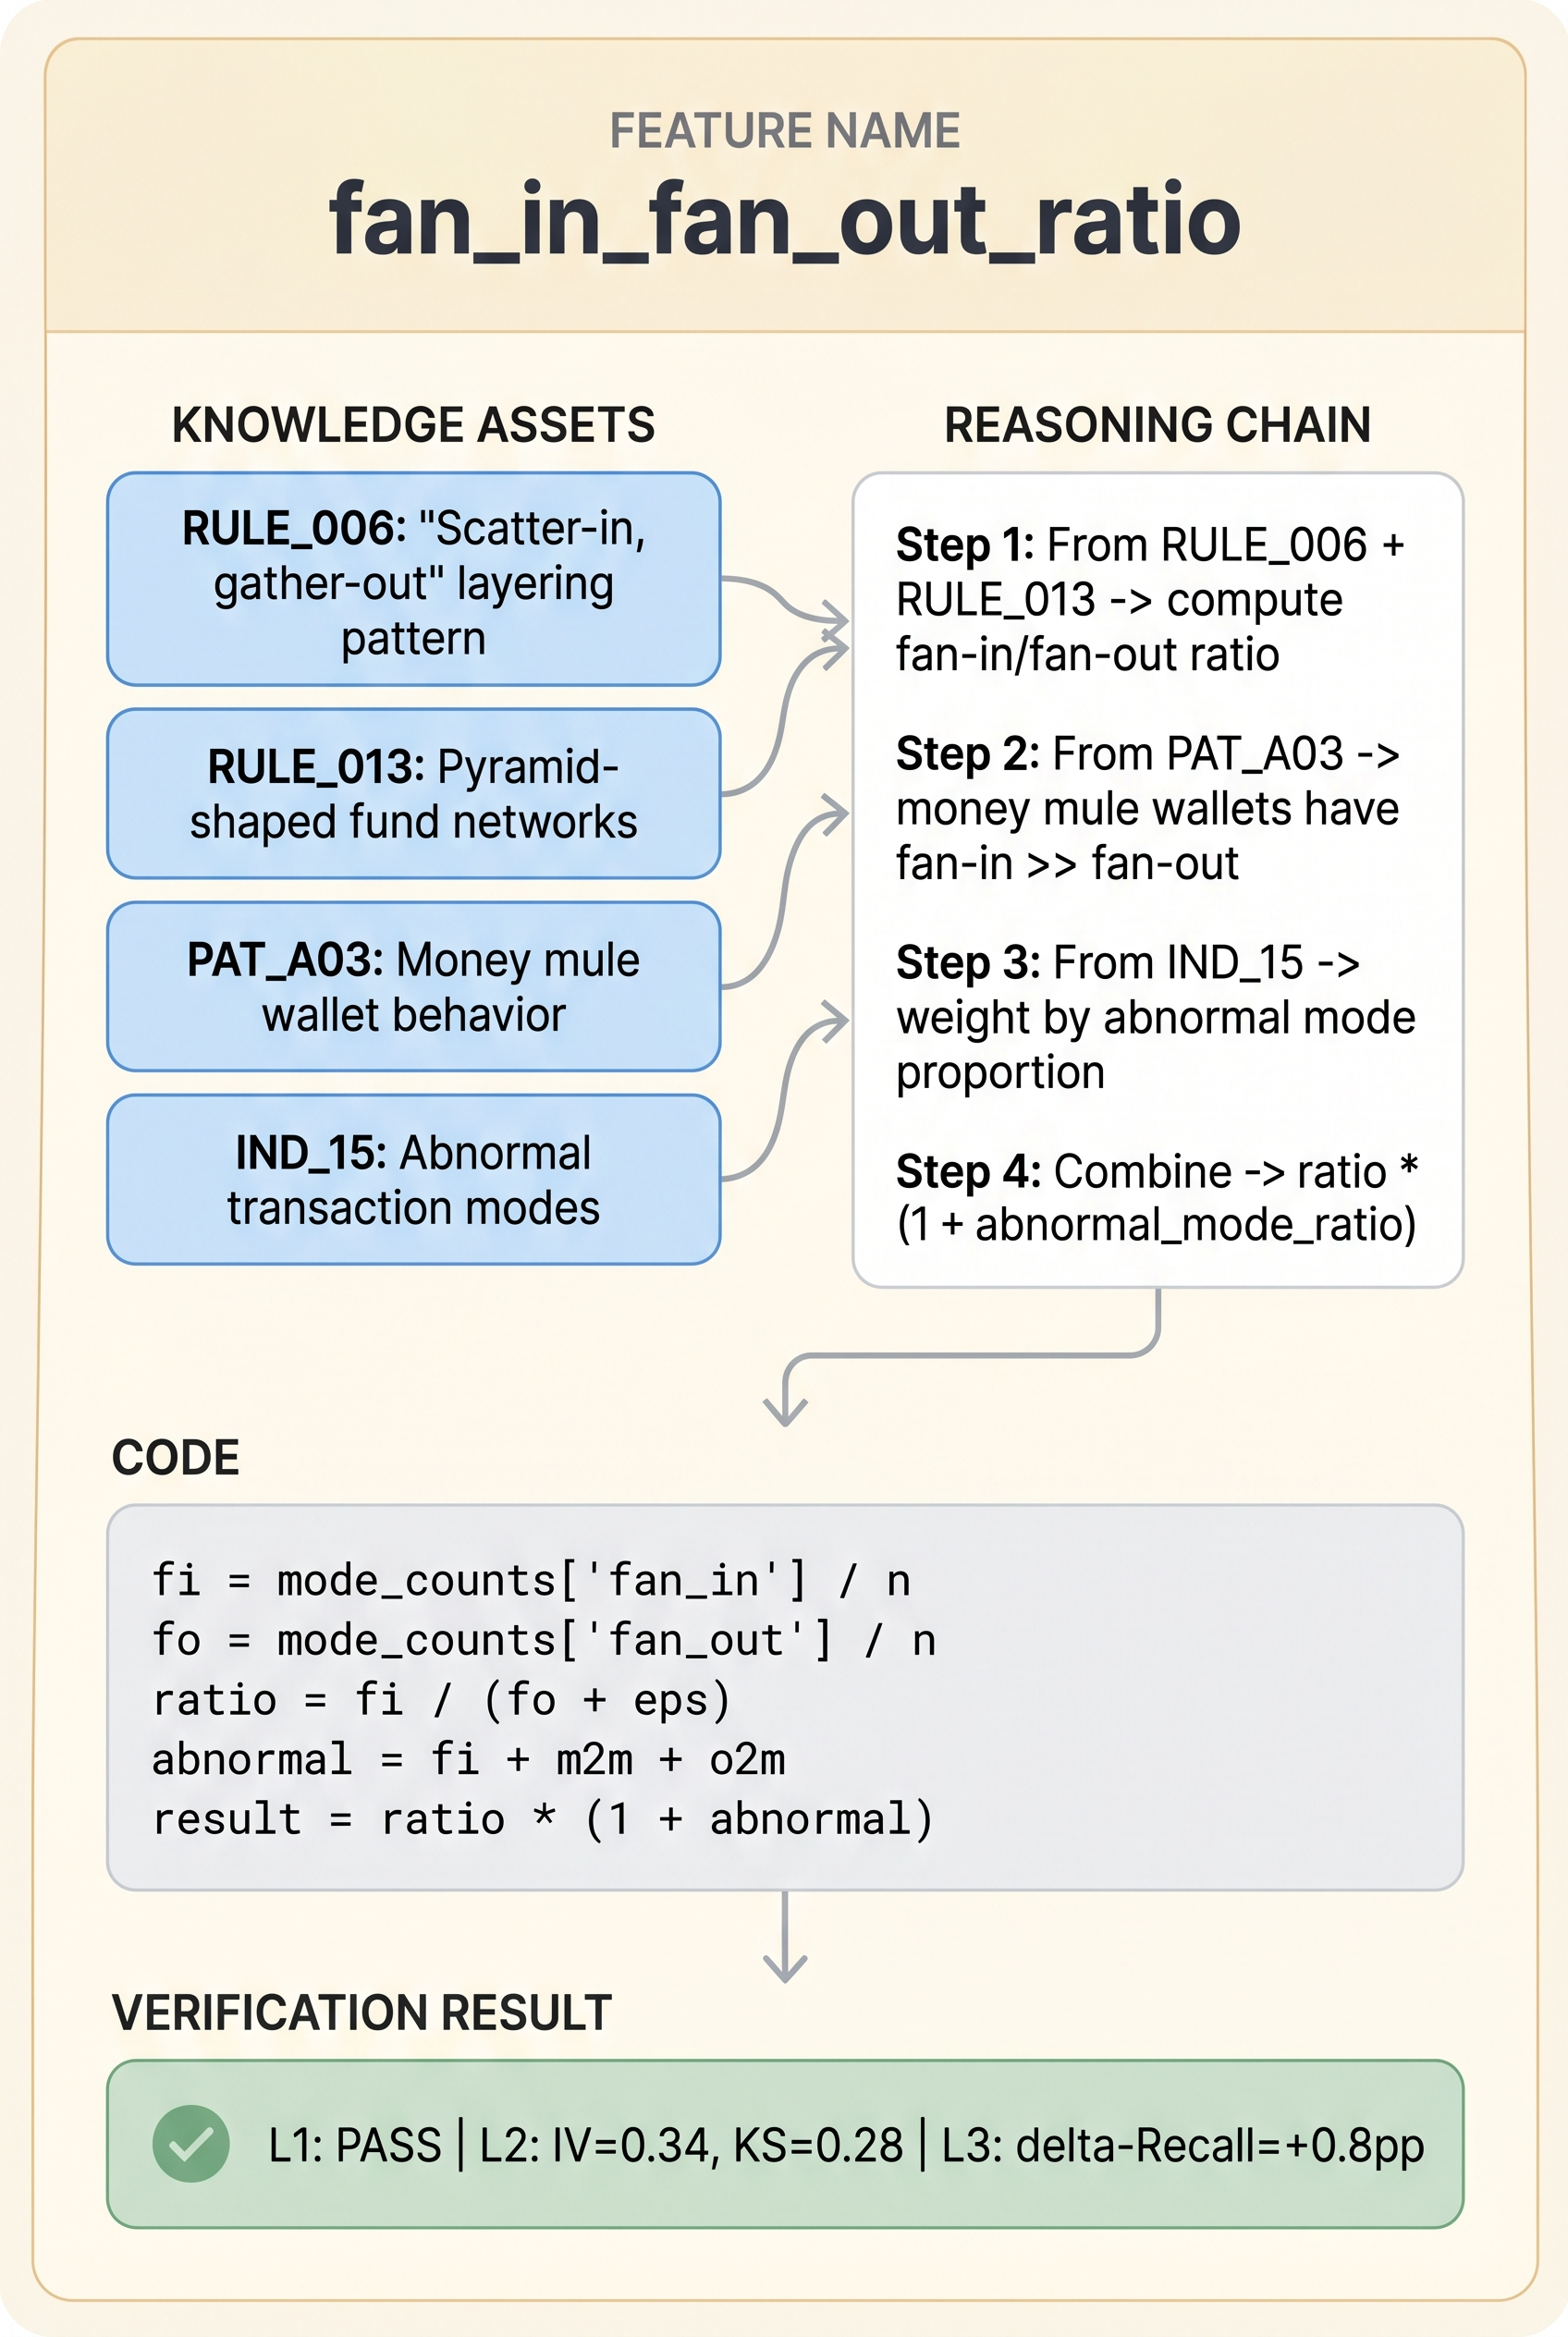
\includegraphics[width=\columnwidth]{figures/provenance_card.png}
    \caption{Provenance card for \texttt{fan\_in\_fan\_out\_ratio}, recording knowledge assets, reasoning chain, generated code, and verification results. Each field enables regulatory audit.}
    \label{fig:provenance}
\end{figure}

\textbf{Case 1: Fan-In/Fan-Out Ratio.}
This feature captures network topology asymmetry by fusing four knowledge assets spanning three types: \textit{RULE\_006} (scatter-in/gather-out layering), \textit{RULE\_013} (pyramid fund networks), \textit{PAT\_A03} (money mule pattern), and \textit{IND\_15} (abnormal transaction modes). The reasoning chain: because RULE\_006/013 indicate directional imbalance in fund flows, compute the fan-in/fan-out mode ratio per wallet; because IND\_15 flags abnormal modes, weight by abnormal mode proportion: $\text{ratio} \times (1 + \text{abnormal\_mode\_ratio})$. No syntactic method would produce this feature---it requires understanding that directional imbalance combined with abnormal mode prevalence characterizes money mule behavior.

\textbf{Case 2: Cross-Dimensional Risk Interaction.}
This feature multiplies geographic risk with temporal anomaly, guided by three knowledge assets: \textit{RULE\_005/014} (cross-regional border flows), \textit{IND\_08/09} (off-hour concentration), and \textit{EXP\_05} (``border region + nighttime = cross-border laundering''). Neither geographic nor temporal signal alone is sufficient; the expert opinion prescribes their conjunction: $\text{is\_high\_risk\_region} \times \text{off\_hour\_ratio}$. This demonstrates \emph{cross-dimensional interaction}: geographic context combined with temporal patterns, where the multiplicative form ensures only the conjunction triggers a high score.

Both features carry complete provenance chains for regulatory audit, a capability absent from all baselines.
